\section{量化误差}
\label{sec:quant-error}

前几节只用平均失真一个数评价量化器。误差本身是一个随机变量，记为
\[
 E=Q(X)-X .
\]
关于它还可以问三个问题：典型的大小是多少，偶尔会大到什么程度，它与读数之间有什么关系。第一个问题决定平均失真，第二个问题关系到最坏情形，第三个问题关系到能否把量化看成“读数加上一点独立噪声”。这一节对已经构造的量化器回答这三个问题，并说明加入共享的随机扰动怎样改变第三个问题的答案。

\subsection{舍入误差与过载误差}
\label{sec:quant-granular-overload}

考虑第~\ref{sec:quant-uniform}节的均匀量化器：$N$个点、步长$\Delta$、范围$[-L,L]$，$L=N\Delta/2$，范围外饱和。按读数是否落在范围内，把平均失真分成两部分：
\begin{equation}
 D=\underbrace{\mathbb{E}\bigl[E^{2}\mathbf{1}_{\{\lvert X\rvert\leq L\}}\bigr]}_{D_{\mathrm{gran}}}+\underbrace{\mathbb{E}\bigl[E^{2}\mathbf{1}_{\{\lvert X\rvert>L\}}\bigr]}_{D_{\mathrm{over}}} .
 \label{eq:quant-granular-overload}
\end{equation}
第一部分是舍入误差的贡献，第二部分是过载误差的贡献。

\paragraph{误差随读数的变化}
图~\ref{fig:quant-error-shape}左图画出$N=8$、$\Delta=1$时误差随读数的变化。范围内误差是锯齿形，在每个区间内从$+\tfrac12$线性降到$-\tfrac12$；范围外误差随读数线性增长，没有上界。

\begin{BookInlineFigure}
 \centering
 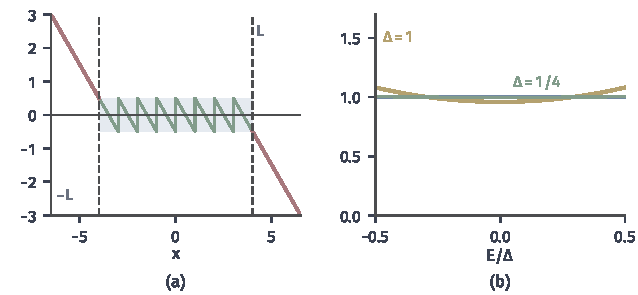
\includegraphics[width=108mm]{figures/07-probability/05-source-coding/matplotlib/quant-error-shape/figure.pdf}
 \caption{均匀量化的误差。(a) $N=8$、$\Delta=1$时$E=Q(x)-x$随读数的变化：范围内（浅蓝带，$\lvert E\rvert\leq\frac12$）为绿色锯齿，范围外为红色直线。(b) 对$\operatorname{Laplace}(0,1)$读数，在不过载的条件下$E/\Delta$的精确密度：黄线为$\Delta=1$（$N=8$），绿线为$\Delta=1/4$（$N=32$），两者范围同为$[-4,4]$；蓝线为均匀密度$1$。}
 \label{fig:quant-error-shape}
\end{BookInlineFigure}

\paragraph{舍入误差}
范围内的读数与所在区间的中点相距不超过$\Delta/2$，所以总有
\[
 D_{\mathrm{gran}}\leq\frac{\Delta^{2}}{4}\,\mathbb{P}\bigl(\lvert X\rvert\leq L\bigr) .
\]
这个界对任何分布都成立，但通常偏大四倍左右。

更常用的是一个近似。若密度在每个区间内几乎不变，那么在读数落在某个区间的条件下，它近似均匀分布于这个区间，误差近似均匀分布于$[-\Delta/2,\Delta/2]$。对均匀分布直接积分，
\[
 \frac{1}{\Delta}\int_{-\Delta/2}^{\Delta/2}e^{2}\,\mathrm{d}e=\frac{\Delta^{2}}{12} .
\]
把各区间合起来，得到
\begin{equation}
 D_{\mathrm{gran}}\approx\frac{\Delta^{2}}{12}\,\mathbb{P}\bigl(\lvert X\rvert\leq L\bigr) .
 \label{eq:quant-granular-approx}
\end{equation}
这称为\term{高分辨率近似}（high-resolution approximation）。它不是精确公式：条件是密度在区间尺度上变化很小，$\Delta$越小越准确。

近似的偏差可以用质心条件看清楚。由引理~\ref{lem:quant-centroid}，一个区间内以中点$c_j$为重构值的条件平方误差，等于条件方差加上质心与中点距离的平方。以Laplace读数的区间$[0,1)$为例，在$0\leq X<1$的条件下，由式~\eqref{eq:quant-laplace-centroid}与二阶矩的积分，得到
\[
 \operatorname{Var}(X\mid0\leq X<1)=0.0793,\qquad (0.5-0.4180)^{2}=0.0067 .
\]
二者相加为$0.0860$，而均匀近似给出$\tfrac1{12}=0.0833$。条件方差比$\tfrac1{12}$小，因为质量偏向区间左端；但重构值不在质心，又多出一项。图~\ref{fig:quant-error-shape}右图画出了合起来的效果：$\Delta=1$时误差的密度在$0.96$到$1.08$之间起伏，$\Delta=1/4$时已几乎是常数$1$。

非均匀量化器的区间长度$\Delta_j$各不相同，式~\eqref{eq:quant-granular-approx}相应地改为
\[
 D_{\mathrm{gran}}\approx\sum_{j}\frac{p_j\Delta_j^{2}}{12} .
\]
概率$p_j$大的区间若取得窄，就能减小这个和；这正是Lloyd--Max量化器在中央划得细的原因。

\paragraph{过载误差}
对Laplace读数，过载部分有显式公式。看右侧：读数$X>L$时报出$c_N=L-\Delta/2$，误差的绝对值是$(X-L)+\Delta/2$。在$X>L$的条件下，超出量$X-L$服从$\operatorname{Exp}(1)$，记为$Z$。对$a=\Delta/2$，
\[
 \mathbb{E}\bigl[(Z+a)^{2}\bigr]=\mathbb{E}[Z^{2}]+2a\,\mathbb{E}[Z]+a^{2}=2+2a+a^{2} .
\]
右侧过载的概率是$\mathrm{e}^{-L}/2$，左右对称，于是
\begin{equation}
 D_{\mathrm{over}}=\mathrm{e}^{-L}\Bigl(\frac{\Delta^{2}}{4}+\Delta+2\Bigr),\qquad L=\frac{N\Delta}{2} .
 \label{eq:quant-laplace-overload}
\end{equation}
它随$L$指数衰减。尾部越轻，过载误差衰减越快；尾部更重的分布，例如按幂律衰减的分布，需要更大的范围才能把过载压下去。

\paragraph{步长的权衡}
把$N=8$代入，$L=4\Delta$。由式~\eqref{eq:quant-granular-approx}与式~\eqref{eq:quant-laplace-overload}，
\[
 D(\Delta)\approx\frac{\Delta^{2}}{12}\bigl(1-\mathrm{e}^{-4\Delta}\bigr)+\mathrm{e}^{-4\Delta}\Bigl(\frac{\Delta^{2}}{4}+\Delta+2\Bigr) .
\]
下面算三个步长。$\Delta=0.5$时范围只到$\pm2$，过载占主导：
\[
 D_{\mathrm{gran}}\approx0.0180,\qquad D_{\mathrm{over}}=0.3468 .
\]
$\Delta=1$时两者相当：
\[
 D_{\mathrm{gran}}\approx0.0818,\qquad D_{\mathrm{over}}=0.0595 .
\]
$\Delta=1.5$时范围到$\pm6$，过载几乎消失，舍入占主导：
\[
 D_{\mathrm{gran}}\approx0.1870,\qquad D_{\mathrm{over}}=0.0101 .
\]
三者的总和约为$0.365$、$0.141$和$0.197$。舍入部分的精确值分别为$0.0182$、$0.0845$与$0.2004$，均匀近似在$\Delta=1.5$时偏小约$7\%$。

图~\ref{fig:quant-gran-overload}画出两部分随步长的完整变化。总误差在$\Delta^{*}\approx1.03$处最小，最小值为$0.1435$，此时舍入部分约占$63\%$。在最优点附近，两部分的变化率相互抵消：再缩小步长，过载的增加超过舍入的减少。

\begin{BookInlineFigure}
 \centering
 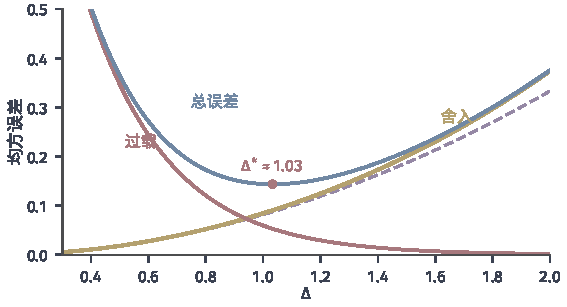
\includegraphics[width=96mm]{figures/07-probability/05-source-coding/matplotlib/quant-gran-overload/figure.pdf}
 \caption{$\operatorname{Laplace}(0,1)$读数、$N=8$的均匀量化器的平均失真随步长的变化，范围$L=4\Delta$。黄线为舍入部分的精确值，紫色虚线为其近似$\frac{\Delta^2}{12}\mathbb{P}(\lvert X\rvert\leq L)$，红线为过载部分~\eqref{eq:quant-laplace-overload}，蓝线为总和；红点为最优步长$\Delta^{*}\approx1.03$。}
 \label{fig:quant-gran-overload}
\end{BookInlineFigure}

\paragraph{点数的权衡}
增加点数时，最优步长与范围一起变化。表~\ref{tab:quant-uniform-points}列出对每个$N$搜索最优步长的结果。点数每加倍，最优范围大约增加$1.1$，而不是保持不变：为了让过载项$\mathrm{e}^{-L}$与舍入项$\Delta^{2}/12$同步减小，范围必须随点数缓慢变宽。所以步长缩小不到一半，每多一个比特，失真只降为原来的$0.35$左右，而不是理想的四分之一。

\begin{BookInlineTable}
 \centering
 \begin{tabular}{rrrrrr}
  \toprule
  $N$ & $\Delta^{*}$ & $L^{*}$ & 舍入 & 过载 & 总失真\\
  \midrule
  $4$ & $1.538$ & $3.08$ & $0.2020$ & $0.1906$ & $0.3926$\\
  $8$ & $1.034$ & $4.13$ & $0.0907$ & $0.0528$ & $0.1435$\\
  $16$ & $0.652$ & $5.22$ & $0.0357$ & $0.0150$ & $0.0507$\\
  $32$ & $0.396$ & $6.34$ & $0.0131$ & $0.0043$ & $0.0174$\\
  \bottomrule
 \end{tabular}
 \caption{$\operatorname{Laplace}(0,1)$读数的最优均匀量化器（定长索引）。舍入与过载为精确值；同样点数的Lloyd--Max量化器失真依次为$0.3524$、$0.1090$、$0.0307$、$0.0082$。}
 \label{tab:quant-uniform-points}
\end{BookInlineTable}

\paragraph{误差的尾部}
平均失真之外，有时还关心误差偶尔有多大。范围内的误差总不超过$\Delta/2$，超过$\Delta/2$的误差只能来自过载。对$s\geq\Delta/2$，$\lvert E\rvert>s$等价于$\lvert X\rvert>L-\Delta/2+s$，所以
\[
 \mathbb{P}\bigl(\lvert E\rvert>s\bigr)=\mathrm{e}^{-(L-\Delta/2+s)},\qquad s\geq\frac{\Delta}{2} .
\]
$N=8$、$\Delta=1$时，误差超过$0.5$的概率是$\mathrm{e}^{-4}=0.018$，超过$1$的概率是$\mathrm{e}^{-4.5}=0.011$，超过$2$的概率是$\mathrm{e}^{-5.5}=0.004$。误差没有上界，但它的尾部继承了读数的尾部。需要保证最坏误差时，只能加大范围或另外描述越界的读数。

\paragraph{误差与读数的关系}
误差$E=Q(X)-X$是读数的函数，给定读数，误差就完全确定。所以$E$与$X$不可能独立（除非$E$几乎必然为常数）。即使只看相关性，误差与读数一般也相关：若重构值都是质心，由第~\ref{sec:quant-nonuniform}节的正交性，$\mathbb{E}[EQ(X)]=0$，而$X=Q(X)-E$，于是
\[
 \mathbb{E}[XE]=\mathbb{E}[Q(X)E]-\mathbb{E}[E^{2}]=-D .
\]
又$\mathbb{E}[E]=0$，所以$\operatorname{Cov}(X,E)=-D\neq0$。

常用的“加性噪声模型”把量化写成$Q(X)=X+E$，并假定$E$与$X$独立、在$[-\Delta/2,\Delta/2]$上均匀分布。上面的讨论说明这只是一个近似：在高分辨率下，误差的分布接近均匀（图~\ref{fig:quant-error-shape}右图），与读数的相关系数$-\sqrt{D}/\sqrt{\operatorname{Var}(X)}$趋于零，用它估算平均失真是合理的；但在粗量化、有过载，或读数本身取值规则（例如总落在刻度附近、长时间停在同一个区间内）时，它会给出错误的结论。第~\ref{sec:quant-dither}节给出一种使这个模型精确成立的办法。

\paragraph{期望难以计算时}
上面的平均失真都由显式积分得到。分布或区域复杂时，例如向量量化的Voronoi区域，期望难以直接积分，可以用模拟的平均代替：独立地生成$n$个读数，计算误差平方的样本平均。它本身是期望的一个估计，有自己的随机误差，应当与量化误差分开报告。例如对$N=8$、$\Delta=1$的Laplace例子，用$n=10^{5}$个模拟读数（种子7），得到估计$0.1438$，标准误差约$0.0025$；精确值$0.1440$在其范围之内。模拟误差怎样随$n$缩小、怎样给出可靠的区间，见第~\ref{chap:monte-carlo-integration-error}章。

\paragraph{比较的前提}
比较两个量化器时，源分布、失真函数和描述资源必须相同。表~\ref{tab:quant-uniform-points}与图~\ref{fig:quant-operational}都遵守这一点：同一个Laplace读数、平方误差，横向比较时固定点数或固定平均码长。单纯增加点数总能降低误差，但同时增加存储、搜索与描述长度；说一个量化器“更好”，必须说明是在哪种资源下更好。

\subsection{抖动对误差的影响}
\label{sec:quant-dither}

确定性量化的误差由读数决定，这在某些场合是个实际问题。设读数长时间停在$x=0.3$附近，用步长$\Delta=1$、零为重构值的无穷均匀量化器~\eqref{eq:quant-midtread}，每次都报$0$，误差恒为$-0.3$。多次记录再平均也消除不了这个偏差，因为误差没有任何随机性可以被平均掉。能否让误差变成与读数无关的随机量？

\paragraph{减性抖动}
办法是在量化前给读数加一个随机扰动，并让解码器知道同一个扰动，重构时再把它减掉。设$U$与$X$独立，服从$[-\Delta/2,\Delta/2)$上的均匀分布。编码器量化$X+U$，传送索引；解码器取得同一个$U$的值（例如双方使用同一个伪随机数发生器和种子），输出
\begin{equation}
 \hat{X}=Q_{\Delta}(X+U)-U .
 \label{eq:quant-subtractive-dither}
\end{equation}
这称为\term{减性抖动}（subtractive dither），所加的扰动称为\term{抖动}（dither）。重构误差为
\[
 E=\hat{X}-X=Q_{\Delta}(X+U)-(X+U) ,
\]
也就是对$V=X+U$做舍入的误差。

先用$x=0.3$、$\Delta=1$手算三个扰动值。取$u=0.37$，$v=0.67$舍入到$1$，于是
\[
 \hat{x}=1-0.37=0.63,\qquad E=0.33 .
\]
取$u=-0.42$，$v=-0.12$舍入到$0$，于是
\[
 \hat{x}=0+0.42=0.42,\qquad E=0.12 .
\]
取$u=0.1$，$v=0.4$舍入到$0$，于是
\[
 \hat{x}=-0.1,\qquad E=-0.4 .
\]
同一个读数，误差随扰动变化，有正有负。

\paragraph{误差的分布}
为什么误差会均匀？固定$x$，$V=x+U$均匀分布在一个长度恰为$\Delta$的区间$[x-\Delta/2,x+\Delta/2)$上。这个区间恰好跨过一个刻度区间的边界，把它切成两段：左段舍入到一个刻度，右段舍入到下一个刻度。两段上的舍入误差$Q_{\Delta}(v)-v$各自扫过$[-\Delta/2,\Delta/2)$的一部分，拼起来恰好扫过一遍。图~\ref{fig:quant-dither-mechanism}画出$x=0.3$的情形。

\begin{BookInlineFigure}
 \centering
 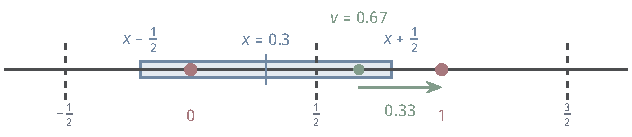
\includegraphics[width=107.1mm]{figures/07-probability/05-source-coding/tikz/quant-dither-mechanism/figure.pdf}
 \caption{减性抖动的机制，$\Delta=1$，$x=0.3$。浅蓝带是$V=x+U$的取值范围$[-0.2,0.8)$，红点是刻度$0$与$1$，虚线是区间边界。带中$[-0.2,0.5)$部分舍入到$0$，误差$-v$取遍$(-0.5,0.2]$；$[0.5,0.8)$部分舍入到$1$，误差$1-v$取遍$(0.2,0.5]$。绿点为$u=0.37$时的$v=0.67$，箭头长度是误差$0.33$。}
 \label{fig:quant-dither-mechanism}
\end{BookInlineFigure}

\begin{theorem}[减性抖动的误差]
\label{thm:quant-subtractive-dither}
设$Q_{\Delta}$为式~\eqref{eq:quant-midtread}的无穷均匀量化器，$U$服从$[-\Delta/2,\Delta/2)$上的均匀分布且与$X$独立。则式~\eqref{eq:quant-subtractive-dither}的重构误差$E=\hat{X}-X$服从$(-\Delta/2,\Delta/2]$上的均匀分布，并且与$X$独立。特别地，
\begin{equation}
 \mathbb{E}[E]=0,\qquad \mathbb{E}[E^{2}]=\frac{\Delta^{2}}{12} ,
 \label{eq:quant-dither-moments}
\end{equation}
对任何读数分布成立。
\end{theorem}

\begin{proof}
记$g(v)=Q_{\Delta}(v)-v$，它是周期为$\Delta$的函数，在$[k\Delta-\Delta/2,k\Delta+\Delta/2)$上等于$k\Delta-v$，取值于$(-\Delta/2,\Delta/2]$。于是$E=g(X+U)$。

先固定$x$，计算$g(x+U)$的分布。$x+U$在$I_x=[x-\Delta/2,x+\Delta/2)$上均匀分布，密度为$1/\Delta$。对$(-\Delta/2,\Delta/2]$中的Borel集$B$，
\[
 \mathbb{P}\bigl(g(x+U)\in B\bigr)=\frac{1}{\Delta}\,\lambda\bigl(\{v\in I_x:g(v)\in B\}\bigr) ,
\]
$\lambda$为长度。$I_x$长度恰为$\Delta$，按刻度区间的边界把它切成至多两段，每段上$g(v)=k\Delta-v$是斜率为$-1$的平移，保持长度。两段的像拼起来恰为$(-\Delta/2,\Delta/2]$，互不重叠，因为$g$的周期为$\Delta$，长度为$\Delta$的区间上每个误差值恰好出现一次。所以上式右边等于$\lambda(B)/\Delta$，与$x$无关。

再证独立性。$X$与$U$独立，$(X,U)$的联合分布是乘积分布。对Borel集$A$与$B$，由Fubini定理先对$U$积分，
\[
 \mathbb{P}(X\in A,\ E\in B)=\int_{A}\mathbb{P}\bigl(g(x+U)\in B\bigr)\,P_X(\mathrm{d}x)=P_X(A)\,\frac{\lambda(B)}{\Delta} .
\]
取$A=\mathbb{R}$，得$E$服从均匀分布；于是上式就是$\mathbb{P}(X\in A)\mathbb{P}(E\in B)$，$E$与$X$独立。式~\eqref{eq:quant-dither-moments}是均匀分布的均值与二阶矩。
\end{proof}

定理把加性噪声模型从近似变成了精确：$\hat{X}=X+E$，$E$与$X$独立且均匀。条件也说得很清楚：抖动必须恰好在一个步长上均匀，必须与读数独立，解码器必须减去同一个抖动，并且量化器不能过载。最后一条对无穷刻度自然成立；若刻度只覆盖$[-L,L]$，则需要$\lvert X\rvert\leq L-\Delta/2$，使$X+U$不越出范围。

回到$x=0.3$的例子。不加抖动时误差恒为$-0.3$，平方误差$0.09$；加减性抖动后，误差的均值为$0$、均方为$\tfrac1{12}\approx0.083$。图~\ref{fig:quant-dither-mse}右图用$20000$个抖动值（种子4）模拟了这个读数的误差：直方图在$[-0.5,0.5]$上是平的，样本均值约为$0.0004$，均方约为$0.0831$。

\paragraph{代价与资源}
抖动并不减小平均失真，它改变的是误差的结构。对一个读数分布，不加抖动的平均失真可能比$\Delta^{2}/12$小，也可能大。例如Laplace读数、$\Delta=1$时，不加抖动的无穷均匀量化器平均失真为$0.0810$，略小于减性抖动的$0.0833$；若读数总落在刻度上，不加抖动的误差为零，加抖动反而得到$\tfrac1{12}$。换来的好处是：误差与读数独立、无偏，多次独立抖动的记录取平均时误差会被平均掉。

这个方案还用到了额外的资源。给定$U=u$时，编码器仍只发送有限或可数个索引之一，重构值落在平移后的刻度$\{k\Delta-u\}$上；但随着$u$变化，所有可能的重构值铺满了整条实轴，不再是第~\ref{sec:quant-model}节意义下的有限码本。它依赖编码器与解码器共享同一个随机数，这是一种边信息。所以减性抖动是量化模型的一个扩展，与普通量化器比较时，要把共享扰动的要求一并计入。

\paragraph{非减性抖动}
若解码器拿不到抖动，只能输出$Q_{\Delta}(X+U)$，称为\term{非减性抖动}（non-subtractive dither）。这时误差不再与读数独立。固定读数$x=k\Delta+s$，$0\leq s<\Delta$，量化输出只可能是$k\Delta$或$(k+1)\Delta$；后者发生当且仅当$U\geq\Delta/2-s$，概率为$s/\Delta$。于是给定读数的条件均值为
\[
 \mathbb{E}\bigl[Q_{\Delta}(x+U)\bigr]=k\Delta+\frac{s}{\Delta}\Delta=x ,
\]
输出是无偏的。条件均方误差为
\[
 \frac{s}{\Delta}(\Delta-s)^{2}+\Bigl(1-\frac{s}{\Delta}\Bigr)s^{2}=s(\Delta-s) ,
\]
它随读数在$0$与$\Delta^{2}/4$之间变化：读数在刻度上时为$0$，在两刻度正中时达到$\Delta^{2}/4$。若$s$在$[0,\Delta)$上均匀，平均为$\Delta^{2}/6$，是减性抖动的两倍。

\begin{BookInlineFigure}
 \centering
 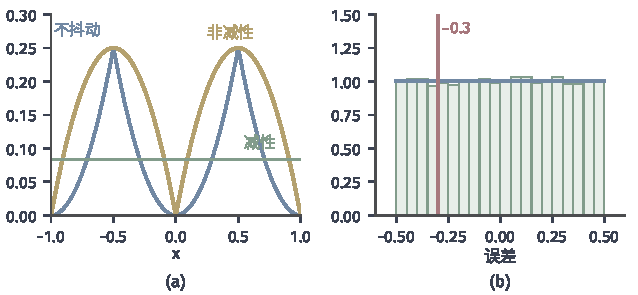
\includegraphics[width=108mm]{figures/07-probability/05-source-coding/matplotlib/quant-dither-mse/figure.pdf}
 \caption{$\Delta=1$的无穷均匀量化器在三种方式下的误差。(a) 给定读数$x$的条件均方误差：蓝线为不加抖动$(x-Q_1(x))^2$，绿线为减性抖动$\frac1{12}$，黄线为非减性抖动$s(1-s)$，$s=x-\lfloor x\rfloor$。(b) $x=0.3$时减性抖动的误差，$20000$个抖动值（种子4）的直方图（浅绿）与均匀密度（蓝线）；红线为不加抖动时的固定误差$-0.3$。}
 \label{fig:quant-dither-mse}
\end{BookInlineFigure}

图~\ref{fig:quant-dither-mse}左图把三种方式放在一起。不加抖动时，条件均方误差在刻度上为零、在刻度中点达到$\Delta^{2}/4$，形状完全由读数决定；非减性抖动消除了偏差，但条件均方误差仍随读数起伏，而且整体更大；只有减性抖动使条件均方误差与读数无关。三者的差别在于误差中有多少成分由读数决定，而这取决于解码器知道多少关于扰动的信息。
